\documentclass[border=10pt]{standalone}

\usepackage{tikz}
\usepackage{tikzsymbols}
\usetikzlibrary{calc,patterns,shapes.geometric}

\def\centerarc[#1](#2)(#3:#4:#5){\draw[#1] ($(#2)+({#5*cos(#3)},{#5*sin(#3)})$) arc (#3:#4:#5);}

\begin{document}
	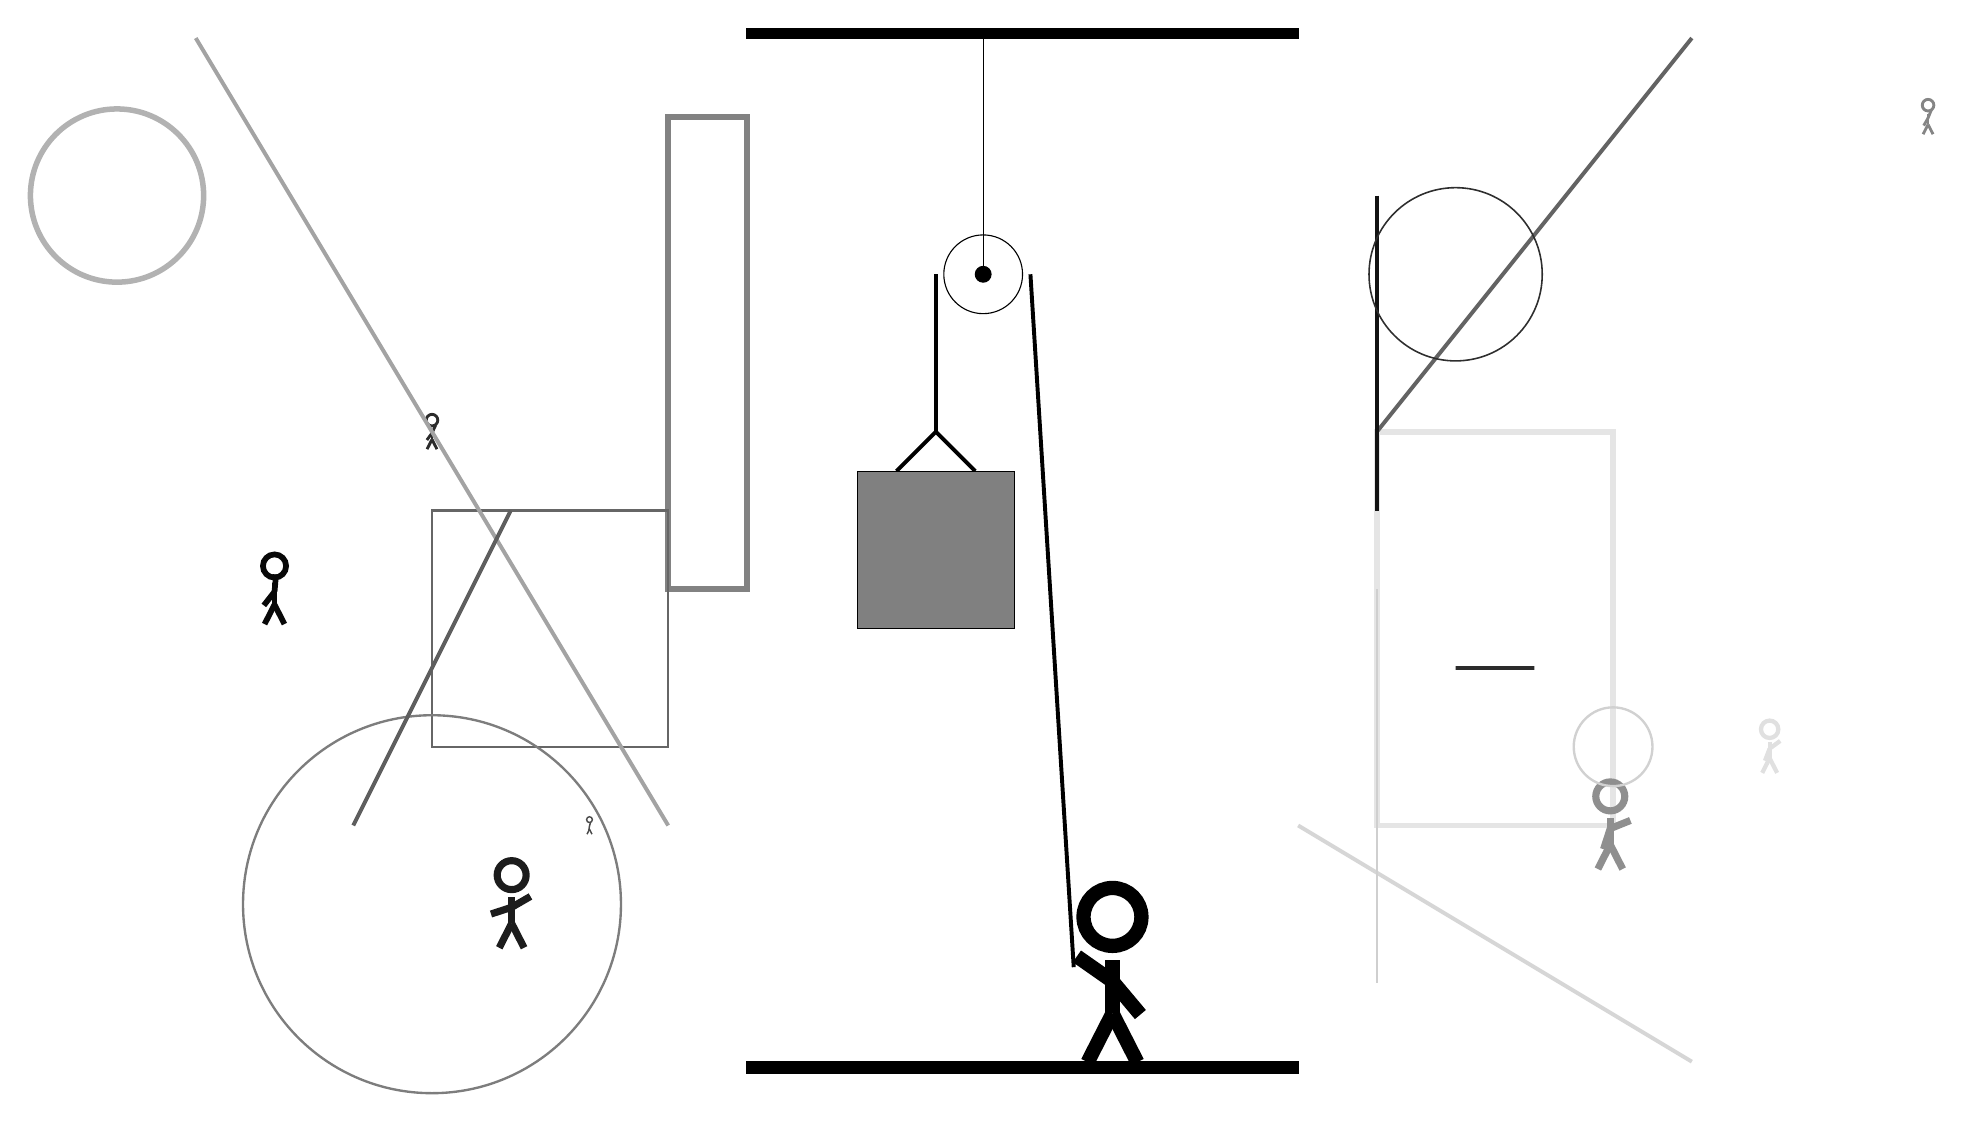
\begin{tikzpicture}
		%%%%% START %%%%%
		
		\draw[fill=black] (-2, 10) rectangle (5, 10.125);
		
		\draw (1, 7) circle (0.5);
		\draw[fill=black] (1, 7) circle (0.1);
		\draw (1, 10) -- (1, 7);
		
		\draw[line width=0.5mm] (-0.1, 4.5) -- (0.4, 5.0) -- (0.9, 4.5);
		\draw[fill=black!50] (-0.6, 4.5) rectangle (1.4, 2.5);
		
		\node[line width=0.2mm, color=black!83] at (-6, 5) {\Strichmaxerl[2][54][65]};
		
		\draw[line width=0.7mm, color=black!49] (-3, 3) rectangle (-2, 9);
		\draw[line width=0.3mm, color=black!60] (-3, 1) rectangle (-6, 4);
		\draw[line width=0.7mm, color=black!10] (6, 0) rectangle (9, 5);
		\draw [line width=0.3mm, color=black!51](-6, -1) circle (2.4);
		\draw[line width=0.5mm, color=black!61](10, 10) -- (6, 5);
		\draw[line width=0.6mm, color=black!83] (7, 2) rectangle (8, 2);
		
		\draw[line width=0.5mm, color=black!16](10, -3) -- (5, 0);
		\draw[line width=0.5mm, color=black!93](6, 8) -- (6, 4);
		\draw[line width=0.2mm, color=black!19] (6, 3) rectangle (6, -2);
		\node[line width=0.5mm, color=black!71] at (-4, 0) {\Strichmaxerl[1][81][74]};
		\node[line width=0.7mm, color=black!48] at (13, 9) {\Strichmaxerl[2][60][68]};
		\draw [line width=0.7mm, color=black!30](-10, 8) circle (1.1);
		\node[line width=0.6mm, color=black!44] at (9, 0) {\Strichmaxerl[5][72][22]};
		\node[line width=0.5mm, color=black!89] at (-5, -1) {\Strichmaxerl[5][18][30]};
		\draw [line width=0.3mm, color=black!18](9, 1) circle (0.5);
		
		\draw[line width=0.5mm, color=black!36](-3, 0) -- (-9, 10);
		\node[line width=0.3mm, color=black!12] at (11, 1) {\Strichmaxerl[3][69][36]};
		\node[line width=0.3mm, color=black!97] at (-8, 3) {\Strichmaxerl[4][52][85]};
		
		\draw[line width=0.5mm, color=black!63](-5, 4) -- (-7, 0);
		\draw [line width=0.2mm, color=black!82](7, 7) circle (1.1);
		
		
		\draw[line width=0.5mm] (0.4, 7) -- (0.4, 5.0);
		\centerarc[line width=0.5mm](1, 7)(0:180:0.6);
		\draw[line width=0.5mm](1.6, 7) -- (2.15, -1.8);
		
		\node at (2.6, -1.9) {\Strichmaxerl[10][-35][-50]};
		
		\draw[fill=black] (-2, -3) rectangle (5, -3.15);
		
		%%%%% END %%%%%
	\end{tikzpicture}
\end{document}